\documentclass[12pt, a4paper]{article}

% ── Packages ─────────────────────────────────────────────────────────────────
\usepackage[T1]{fontenc}
\usepackage[utf8]{inputenc}
\usepackage{lmodern}
\usepackage{microtype}
\usepackage[top=2.5cm, bottom=2.5cm, left=3cm, right=3cm]{geometry}
\setlength{\headheight}{13.6pt}
\addtolength{\topmargin}{-1.6pt}
\usepackage{amsmath, amssymb}
\usepackage{booktabs}
\usepackage{array}
\usepackage{multirow}
\usepackage{graphicx}
\usepackage{caption}
\usepackage{subcaption}
\usepackage{fancyhdr}
\usepackage{parskip}
\usepackage{enumitem}
\usepackage{titlesec}
\usepackage{listings}
\usepackage{makecell}
\usepackage[hidelinks]{hyperref}

% ── Section formatting ────────────────────────────────────────────────────────
\titleformat{\section}{\large\bfseries}{\thesection.}{0.5em}{}[\titlerule]
\titleformat{\subsection}{\normalsize\bfseries}{\thesubsection.}{0.5em}{}
\titleformat{\subsubsection}{\normalsize\itshape}{\thesubsubsection.}{0.5em}{}

% ── Header / Footer ───────────────────────────────────────────────────────────
\pagestyle{fancy}
\fancyhf{}
\rhead{\small Korean Food Freshness Classification}
\lhead{\small Preliminary Report --- 2026}
\cfoot{\thepage}
\renewcommand{\headrulewidth}{0.4pt}

% ── Graphics path ─────────────────────────────────────────────────────────────
\graphicspath{{figures/}}

% ── Code style ────────────────────────────────────────────────────────────────
\lstset{
    basicstyle=\small\ttfamily,
    frame=single,
    language=Python,
    breaklines=true,
    showstringspaces=false,
    numbers=none,
}

% ── Caption setup ─────────────────────────────────────────────────────────────
\captionsetup{font=small, labelfont=bf, skip=6pt}

% ── Table column types ────────────────────────────────────────────────────────
\newcolumntype{L}[1]{>{\raggedright\arraybackslash}p{#1}}
\newcolumntype{C}[1]{>{\centering\arraybackslash}p{#1}}

% ─────────────────────────────────────────────────────────────────────────────
\begin{document}

% ── Title Page ────────────────────────────────────────────────────────────────
\begin{titlepage}
\centering
\vspace*{2.5cm}

{\LARGE\bfseries Freshness Classification of Korean Food}\\[3.5cm]

{\normalsize Digital Image Processing}\\[0.4em]
{\normalsize 2026}\\[3cm]

\hrule
\end{titlepage}

\tableofcontents
\newpage

% ─────────────────────────────────────────────────────────────────────────────
\section{Datasets}
% ─────────────────────────────────────────────────────────────────────────────

\subsection{Available Datasets}

Seven publicly available datasets were identified and surveyed.
Table~\ref{tab:datasets} summarizes their properties.
Together they cover fruits, vegetables, and citrus varieties, with fresh/rotten
binary labels and, in one case, a three-class annotation including formalin-mixed
samples.
One dataset (Ripening Stages) uses an object detection format (YOLOv5) rather
than image classification and is therefore excluded from training experiments.

\begin{table}[h]
\centering
\caption{Datasets surveyed. $^{\dagger}$Object detection format --- excluded from classification experiments.}
\label{tab:datasets}
\begin{tabular}{L{2.8cm} L{3.2cm} C{2.4cm} C{1.3cm} C{1.3cm} C{1.2cm}}
\toprule
\textbf{Dataset} & \textbf{Categories} & \textbf{Classes} & \textbf{Images} & \textbf{Size} & \textbf{Source} \\
\midrule
FruitVision
    & Apple, Banana, Grape, Mango, Orange
    & Fresh / Formalin / Rotten
    & 10,154 & 857 MB & Mendeley \\[4pt]
Lemon Varieties
    & 7 lemon varieties
    & Fresh / Rotten
    & 1,956 & 1.35 GB & Mendeley \\[4pt]
Ripening Stages$^{\dagger}$
    & Strawberry, Avocado
    & Unripe / Partial / Ripe / Rotten
    & --- & 1.97 GB & Mendeley \\[4pt]
Fruits Classification
    & Peach, Pomegranate, Strawberry
    & Fresh / Rotten
    & 1,655 & 14.5 MB & Mendeley \\[4pt]
Fruits Quality
    & 12 mixed fruits
    & Fresh / Rotten
    & 359 & 12.4 MB & Kaggle \\[4pt]
Fruits Fresh/Rotten
    & Apple, Banana, Orange
    & Fresh / Rotten
    & 13,599 & 1.95 GB & Kaggle \\[4pt]
Fresh \& Stale
    & Apple, Banana, Cucumber, Okra, Orange, Potato, Tomato
    & Fresh / Rotten
    & 27,317 & 3.09 GB & Kaggle \\
\midrule
\multicolumn{3}{l}{\textbf{Total (classification datasets)}}
    & \textbf{55,040} & & \\
\bottomrule
\end{tabular}
\end{table}

\subsection{Dataset Sources}

\begin{itemize}[leftmargin=*, itemsep=2pt]
    \item \textbf{FruitVision} ---
    \url{https://data.mendeley.com/datasets/xkbjx8959c/2}

    \item \textbf{Lemon Varieties} ---
    \url{https://data.mendeley.com/datasets/mygrsk3vyb/2}

    \item \textbf{Ripening Stages} ---
    \url{https://data.mendeley.com/datasets/mygrsk3vyb/2}

    \item \textbf{Fruits Classification} ---
    \url{https://data.mendeley.com/datasets/rg254yr63x/1}

    \item \textbf{Fruits Quality} ---
    \url{https://www.kaggle.com/datasets/nourabdoun/fruits-quality-fresh-vs-rotten}

    \item \textbf{Fruits Fresh/Rotten} ---
    \url{https://www.kaggle.com/datasets/sriramr/fruits-fresh-and-rotten-for-classification}

    \item \textbf{Fresh \& Stale} ---
    \url{https://www.kaggle.com/datasets/swoyam2609/fresh-and-stale-classification}
\end{itemize}


\subsection{Korean Food Dataset --- Proposal}

No labeled dataset for Korean food freshness currently exists in public
repositories.
Table~\ref{tab:korean} lists the target food categories and classification
states for the proposed dataset.

\begin{table}[h]
\centering
\caption{Target categories for the proposed Korean food freshness dataset.}
\label{tab:korean}
\begin{tabular}{L{3cm} C{2.5cm} C{3.2cm} L{4cm}}
\toprule
\textbf{Category} & \textbf{Romanization} & \textbf{States} & \textbf{Notes} \\
\midrule
Kimchi           & kimchi  & Fresh / Rotten             & Color and mold during spoilage \\
Rice cake        & tteok   & Fresh / Rotten             & Mold visible on surface \\
Side dishes      & banchan & Fresh / Rotten             & Vegetable-based, wilting \\
Cooked rice      & bap     & Fresh / Rotten             & Mold indicator \\
Mandarin (Jeju)  & gyul    & Fresh / Semifresh / Rotten & Jeju variety, citrus \\
Strawberry       & ttalgi  & Fresh / Rotten             & Fast spoilage \\
\bottomrule
\end{tabular}
\end{table}

% ─────────────────────────────────────────────────────────────────────────────
\section{Methodology}
% ─────────────────────────────────────────────────────────────────────────────

\subsection{Overall Pipeline}

The classification pipeline consists of four sequential stages:

\begin{center}
\begin{tabular}{clL{7.5cm}}
\toprule
\textbf{Stage} & \textbf{Component} & \textbf{Description} \\
\midrule
1 & Data preparation   & Raw datasets reorganized into unified
                          \texttt{food/state/} folder structure \\
2 & Feature extraction & Pre-trained CNN backbone (ImageNet weights),
                          frozen or partially unfrozen \\
3 & Projection head    & $d_\text{out} \!\to\! 256 \!\to\! 128$
                          linear projection with ReLU \\
4 & Classification     & Linear layer $128 \!\to\! C$
                          with cross-entropy loss \\
\bottomrule
\end{tabular}
\end{center}

All input images are resized to $224 \times 224$ pixels.
Training images undergo data augmentation (random resized crop, horizontal flip,
$\pm 30^{\circ}$ rotation, color jitter on brightness/contrast/saturation/hue,
Gaussian blur) to increase robustness to lighting and viewpoint variation.
Validation images are center-cropped without augmentation.
All images are normalized with ImageNet channel statistics
($\mu = [0.485, 0.456, 0.406]$, $\sigma = [0.229, 0.224, 0.225]$).

\subsection{Backbone Architectures}

Four backbone architectures are considered.
Table~\ref{tab:backbones} summarizes their properties.
Experiments are conducted with ResNet-18, MobileNetV3-Small, EfficientNet-B0, and EfficientNet-B2.
EfficientNet-B0 is identified as the recommended architecture for the final
Korean food classifier based on its accuracy-to-parameter ratio and demonstrated
suitability for small datasets.

\begin{table}[h]
\centering
\caption{Backbone architectures considered in this study.}
\label{tab:backbones}
\begin{tabular}{lC{2cm}C{2cm}C{2cm}}
\toprule
\textbf{Model} & \textbf{Params} & \textbf{Out dim} & \textbf{Family} \\
\midrule
ResNet-18       & 11.2M &  512 & ResNet       \\
MobileNetV3-S   &  2.5M &  576 & MobileNet    \\
EfficientNet-B0 &  5.3M & 1280 & EfficientNet \\
EfficientNet-B2 &  9.1M & 1408 & EfficientNet \\
\bottomrule
\end{tabular}
\end{table}

\subsection{Training Conditions}

Four training conditions form an ablation study to determine the optimal degree
of backbone fine-tuning.
Conditions C3 and C4 (with projection head) are the focus of this study,
as the additional non-linear projection consistently improves performance over
a direct linear probe.

\begin{table}[h]
\centering
\caption{Training conditions (ablation study).}
\label{tab:conditions}
\begin{tabular}{llllL{4cm}}
\toprule
\textbf{ID} & \textbf{Name} & \textbf{Backbone} & \textbf{Head} &
\textbf{Description} \\
\midrule
C1 & \texttt{frozen}       & Frozen      & Linear only         & No backbone adaptation \\
C2 & \texttt{layer4}       & Layer4 free & Linear only         & Partial fine-tuning, no projection \\
C3 & \texttt{head\_frozen} & Frozen      & Projection + Linear & Full head, frozen backbone \\
C4 & \texttt{head\_layer4} & Layer4 free & Projection + Linear & Full head + partial fine-tuning \\
\bottomrule
\end{tabular}
\end{table}

In all conditions the backbone is initialized with ImageNet pre-trained weights
and produces a feature vector of dimension $d_\text{out}$ (e.g.\ 512 for
ResNet-18, Table~\ref{tab:backbones}).

\textbf{C1 -- frozen backbone, linear head.}
All backbone weights are frozen; gradients do not flow through the convolutional
layers.
A single linear layer $d_\text{out} \to C$ is trained from scratch.
This is the classical \emph{linear probe} setting, where the pre-trained backbone
acts purely as a fixed feature extractor.

\textbf{C2 -- layer4 unfrozen, linear head.}
The last residual block of the backbone (\texttt{layer4} in ResNet notation,
comprising two residual units totaling $\approx$\,2M parameters for ResNet-18)
is unfrozen and fine-tuned jointly with the linear head.
All earlier layers remain frozen.
This allows the backbone to specialize its high-level features to the target
domain without the cost of full fine-tuning.

\textbf{C3 -- frozen backbone, projection head.}
A two-layer non-linear projection head
($d_\text{out} \!\to\! 256 \!\to\! 128$ with ReLU) is appended before the
final linear classifier.
The backbone remains completely frozen; only the head is trained.
The additional capacity of the projection layers allows the model to learn a
more discriminative embedding space without modifying the backbone.

\textbf{C4 -- layer4 unfrozen, projection head.}
Combines the projection head of C3 with the partial fine-tuning of C2.
The last backbone block (\texttt{layer4}) and the full projection head are
optimized jointly, with a lower learning rate applied to the backbone
($\text{lr}_\text{backbone} = 10^{-5}$) to prevent catastrophic forgetting.
This is the most expressive configuration and achieves the best validation F1
for ResNet-18.
A key empirical finding of this study (Section~\ref{sec:fruitstate}) is that the
optimal condition is backbone-dependent: ResNet-18 favors C4, whereas
MobileNetV3 and both EfficientNet variants consistently peak at C3
(frozen backbone + projection head), where their richer feature vectors are
already discriminative enough that backbone fine-tuning offers no further gain
and only risks overfitting.

All models are trained with Adam optimizer
($\text{lr} = 10^{-3}$, $\text{lr}_\text{backbone} = 10^{-5}$,
weight decay $= 10^{-4}$) and cosine annealing over 50 epochs.
Batch size is 32.

\subsection{Label Modes}

Two classification targets are evaluated:

\begin{itemize}
    \item \textbf{state}: classes correspond to freshness states only
    (fresh / rotten, or fresh / formalin / rotten). The model learns
    state-invariant features across all food categories.
    \item \textbf{fruit\_state}: classes correspond to food-state combinations
    (e.g., \texttt{apple\_fresh}, \texttt{apple\_rotten}). The model
    simultaneously learns food identity and freshness state, enabling a richer
    confusion matrix analysis.
\end{itemize}

\subsection{Evaluation Metrics}

Given the potential class imbalance in real-world Korean food datasets,
accuracy alone is insufficient.
Let $TP_c$, $FP_c$, $FN_c$, and $TN_c$ denote true positives, false positives,
false negatives, and true negatives for class $c$, and let $C$ be the total
number of classes.
The following metrics are reported:

\begin{itemize}
    \item \textbf{Accuracy}: fraction of all samples correctly classified,
    \begin{equation}
        \text{Accuracy} = \frac{\displaystyle\sum_{c=1}^{C} TP_c}{\text{total samples}}.
    \end{equation}

    \item \textbf{Precision} (per class): fraction of predicted positives that
    are truly positive,
    \begin{equation}
        \text{Precision}_c = \frac{TP_c}{TP_c + FP_c}.
    \end{equation}

    \item \textbf{Recall} (per class): fraction of actual positives correctly
    identified,
    \begin{equation}
        \text{Recall}_c = \frac{TP_c}{TP_c + FN_c}.
    \end{equation}

    \item \textbf{F1-score} (per class): harmonic mean of precision and recall,
    \begin{equation}
        F1_c = \frac{2\,\cdot\,\text{Precision}_c\,\cdot\,\text{Recall}_c}
                    {\text{Precision}_c + \text{Recall}_c}
             = \frac{2\,TP_c}{2\,TP_c + FP_c + FN_c}.
    \end{equation}

    \item \textbf{Macro averages}: each per-class metric is averaged uniformly
    over all classes,
    \begin{equation}
        \overline{F1} = \frac{1}{C}\sum_{c=1}^{C} F1_c,
        \qquad
        \overline{\text{Precision}} = \frac{1}{C}\sum_{c=1}^{C} \text{Precision}_c,
        \qquad
        \overline{\text{Recall}} = \frac{1}{C}\sum_{c=1}^{C} \text{Recall}_c.
    \end{equation}
    Macro averaging treats every class equally regardless of sample count,
    which is essential when minority classes (e.g.\ formalin) are
    safety-critical.

    \item \textbf{Confusion matrix}: row-normalized per true class, to identify
    systematic misclassification patterns.
\end{itemize}

For food safety applications, recall on the \textit{rotten} class is
particularly critical: a false negative (rotten food classified as fresh)
carries higher risk than a false positive.

% ─────────────────────────────────────────────────────────────────────────────
\section{Preliminary Experiments}
% ─────────────────────────────────────────────────────────────────────────────

\subsection{Setup}

Experiments are organized in three phases.
\textbf{Phase 1} uses ResNet-18 as baseline backbone across all six datasets,
all four conditions (C1--C4), and both label modes (state and fruit\_state).
\textbf{Phase 2} introduces MobileNetV3-Small, EfficientNet-B0, and
EfficientNet-B2 for backbone comparison across conditions C1--C4.
\textbf{Phase 3} targets the two apple/banana/orange and
peach/pomegranate/strawberry collections (KFR and MFR) in fruit\_state mode
(6 classes each) with all four backbones, then combines them into ensembles and
benchmarks the result against published work on the same datasets
(Section~\ref{sec:fruitstate}).
All experiments apply a stratified 80/20 train/validation split with fixed
seed 42 and train for 60 epochs with Adam optimizer and cosine annealing.

\subsection{Results --- Phase 1: ResNet-18 Baseline}

Table~\ref{tab:results_r18} reports the best macro F1-score for ResNet-18
across all datasets and conditions.
C4 (head\_layer4) achieves the best result in most datasets;
C2 (layer4) wins on the smallest dataset (Fruits Quality, 359 images).

\begin{table}[h]
\centering
\caption{Best macro F1-score (\%) --- ResNet-18, all conditions, state mode.
Bold: best per dataset.}
\label{tab:results_r18}
\setlength{\tabcolsep}{5pt}
\begin{tabular}{lC{1.6cm}C{1.6cm}C{1.6cm}C{1.6cm}C{1.8cm}}
\toprule
\textbf{Dataset} & \textbf{C1} & \textbf{C2} & \textbf{C3} & \textbf{C4} & \textbf{Best cond.} \\
\midrule
Fruits Fresh/Rotten & 97.6 & 99.8 & 99.4 & \textbf{99.8} & C2 / C4 \\
Fresh \& Stale      & 95.0 & 98.9 & 98.0 & \textbf{99.0} & C4 \\
Lemon Varieties     & 96.2 & 98.0 & 96.2 & \textbf{98.5} & C4 \\
Fruits Classification & 94.3 & 95.5 & 95.2 & \textbf{96.4} & C4 \\
FruitVision (3-cls) & 78.3 & \textbf{91.0} & 86.7 & 90.6 & C2 \\
Fruits Quality      & 86.1 & \textbf{91.6} & 86.0 & 88.9 & C2 \\
\bottomrule
\end{tabular}
\end{table}

\subsection{Results --- Phase 2: Backbone Comparison}

Table~\ref{tab:results_bb} compares the best F1-score per dataset across all
four backbones (state mode, best condition per cell).
The condition that produced each value is shown in parentheses.

\begin{table}[h]
\centering
\caption{Best macro F1-score (\%) by backbone --- state mode.
Best condition shown in parentheses. Bold: best backbone per dataset.}
\label{tab:results_bb}
\setlength{\tabcolsep}{4pt}
\begin{tabular}{lC{2.1cm}C{2.1cm}C{2.1cm}C{2.1cm}C{1.4cm}}
\toprule
\textbf{Dataset} & \textbf{R18} & \textbf{MN3} & \textbf{EB0} & \textbf{EB2} & \textbf{Winner} \\
\midrule
Fruits Fresh/Rotten   & 99.8 (C4) & \textbf{100.0} (C3) & \textbf{100.0} (C3) & 99.9 (C3) & MN3/EB0 \\
Fresh \& Stale        & 99.0 (C4) & 99.2 (C3) & \textbf{99.4} (C3) & 99.3 (C3) & EB0 \\
Lemon Varieties       & 98.5 (C4) & 98.2 (C3) & \textbf{98.7} (C3) & 98.0 (C3) & EB0 \\
Fruits Classification & 96.4 (C4) & 96.7 (C3) & \textbf{97.0} (C3) & 96.4 (C3) & EB0 \\
FruitVision (3-cls)   & 91.0 (C2) & \textbf{92.4} (C3) & 91.6 (C3) & 92.3 (C3) & MN3 \\
Fruits Quality        & \textbf{91.6} (C2) & \textbf{91.6} (C1) & 86.1 (C4) & 88.9 (C1) & R18/MN3 \\
\bottomrule
\end{tabular}
\end{table}

\paragraph{Optimal condition per backbone.}
A consistent pattern emerges across datasets:
ResNet-18 performs best under C4 (layer4 unfrozen + projection head) in most
datasets, while MobileNetV3-Small and both EfficientNet variants perform best
under C3 (backbone frozen + projection head).
This suggests that the higher-dimensional feature vectors of the
MobileNet/EfficientNet backbones (576--1408 vs.\ 512 for ResNet-18) are already
sufficiently discriminative without fine-tuning, whereas ResNet-18 benefits from
partial backbone adaptation to the target domain.

\paragraph{Effect of dataset size.}
On the smallest dataset (Fruits Quality, 359 images), ResNet-18 outperforms
EfficientNet-B0 by 5.5 percentage points.
On datasets with more than 1,500 images, EfficientNet-B0 consistently matches
or surpasses ResNet-18.
This indicates that EfficientNet's larger head is more prone to overfitting
on very small datasets.

\subsection{All Runs --- ResNet-18 Complete Results}

Table~\ref{tab:allruns} lists all ResNet-18 runs sorted by F1-score.

\begin{table}[h]
\centering
\small
\caption{All ResNet-18 runs sorted by F1-score (state mode, 60 epochs).}
\label{tab:allruns}
\setlength{\tabcolsep}{4pt}
\begin{tabular}{L{3.5cm} C{2.2cm} C{1.2cm} C{1.2cm} C{1.2cm} C{1.2cm}}
\toprule
\textbf{Dataset} & \textbf{Condition} & \textbf{Acc} & \textbf{F1} & \textbf{MCC} & \textbf{AUC} \\
\midrule
Fruits Fresh/Rotten & layer4      & 99.8 & 99.8 & 0.996 & 1.000 \\
Fruits Fresh/Rotten & head\_layer4 & 99.8 & 99.8 & 0.996 & 1.000 \\
Fresh \& Stale      & head\_layer4 & 99.0 & 99.0 & 0.979 & 1.000 \\
Lemon Varieties     & head\_layer4 & 98.5 & 98.5 & 0.970 & 1.000 \\
Fresh \& Stale      & layer4      & 98.9 & 98.9 & 0.978 & 1.000 \\
Fruits Fresh/Rotten & head\_frozen & 99.4 & 99.4 & 0.987 & 0.999 \\
Fresh \& Stale      & head\_frozen & 98.0 & 98.0 & 0.960 & 1.000 \\
Lemon Varieties     & layer4      & 98.0 & 98.0 & 0.960 & 0.999 \\
Fruits Fresh/Rotten & frozen      & 97.6 & 97.6 & 0.952 & 0.997 \\
Fresh \& Stale      & frozen      & 95.0 & 95.0 & 0.899 & 1.000 \\
Fruits Classification & head\_layer4 & 96.4 & 96.4 & 0.929 & 0.995 \\
Lemon Varieties     & frozen      & 96.2 & 96.2 & 0.925 & 0.992 \\
Fruits Classification & layer4    & 95.5 & 95.5 & 0.912 & 0.993 \\
Fruits Classification & head\_frozen & 95.2 & 95.2 & 0.904 & 0.990 \\
Fruits Classification & frozen    & 94.3 & 94.3 & 0.888 & 0.982 \\
FruitVision         & layer4      & 90.9 & 91.0 & 0.863 & 0.981 \\
FruitVision         & head\_layer4 & 90.4 & 90.6 & 0.856 & 0.982 \\
Fruits Quality      & layer4      & 91.7 & 91.6 & 0.839 & 0.947 \\
FruitVision         & head\_frozen & 86.4 & 86.7 & 0.797 & 0.965 \\
Fruits Quality      & head\_layer4 & 88.9 & 88.9 & 0.789 & 0.951 \\
Fruits Quality      & frozen      & 86.1 & 86.1 & 0.732 & 0.914 \\
FruitVision         & frozen      & 78.0 & 78.3 & 0.686 & 0.932 \\
\bottomrule
\end{tabular}
\end{table}

\subsection{Fruit-State Classification and Benchmark vs.\ Published Work}
\label{sec:fruitstate}

To position this work against the literature, the two apple/banana/orange (KFR)
and peach/pomegranate/strawberry (MFR) collections were trained in
\texttt{fruit\_state} mode (6 classes: each fruit $\times$ fresh/rotten) with the
full $4 \times 4$ grid of backbones and conditions.
These two datasets were selected because published papers report results on the
exact same data, enabling a like-for-like comparison.
Tables~\ref{tab:kfr_fs} and~\ref{tab:mfr_fs} report the macro F1-score for every
backbone--condition combination.

\begin{table}[h]
\centering
\caption{KFR (apple/banana/orange) --- macro F1 (\%), fruit\_state mode,
all backbones $\times$ conditions. Bold: best per backbone.}
\label{tab:kfr_fs}
\setlength{\tabcolsep}{6pt}
\begin{tabular}{lC{1.7cm}C{1.7cm}C{1.7cm}C{1.7cm}}
\toprule
\textbf{Backbone} & \textbf{C1} & \textbf{C2} & \textbf{C3} & \textbf{C4} \\
\midrule
ResNet-18       & 97.78 & 99.46 & 99.40 & \textbf{99.65} \\
MobileNetV3-S   & 98.71 & 97.25 & \textbf{100.0} & 99.20 \\
EfficientNet-B0 & 99.70 & 98.75 & \textbf{100.0} & 99.46 \\
EfficientNet-B2 & 99.53 & 98.46 & \textbf{99.97} & 99.36 \\
\bottomrule
\end{tabular}
\end{table}

\begin{table}[h]
\centering
\caption{MFR (peach/pomegranate/strawberry) --- macro F1 (\%), fruit\_state
mode, all backbones $\times$ conditions. Bold: best per backbone.}
\label{tab:mfr_fs}
\setlength{\tabcolsep}{6pt}
\begin{tabular}{lC{1.7cm}C{1.7cm}C{1.7cm}C{1.7cm}}
\toprule
\textbf{Backbone} & \textbf{C1} & \textbf{C2} & \textbf{C3} & \textbf{C4} \\
\midrule
ResNet-18       & 90.98 & 92.67 & \textbf{94.09} & 93.35 \\
MobileNetV3-S   & 93.13 & 89.48 & \textbf{95.25} & 93.84 \\
EfficientNet-B0 & 93.36 & 84.05 & \textbf{95.72} & 88.49 \\
EfficientNet-B2 & 92.82 & 82.08 & \textbf{93.98} & 84.71 \\
\bottomrule
\end{tabular}
\end{table}

The C3 dominance noted for state mode holds even more strongly here: C3 is the
best condition for every backbone except ResNet-18 on both datasets, and the two
best individual models overall (EfficientNet-B0--C3 and MobileNetV3--C3) reach a
perfect 100.0\% macro F1 on KFR.
On the smaller, harder MFR collection the same EfficientNet-B0--C3 leads at
95.72\%.

\paragraph{Comparison with published papers.}
All three reference papers report \emph{accuracy} as their primary metric, so for
a fair comparison our accuracy is used in Table~\ref{tab:benchmark} rather than
macro F1.
On both datasets our models surpass the published state of the art.

\begin{table}[h]
\centering
\caption{Benchmark against published work on the same datasets (metric:
accuracy). Bold: best result per dataset.}
\label{tab:benchmark}
\setlength{\tabcolsep}{4pt}
\begin{tabular}{L{4.6cm} L{3.0cm} C{1.6cm} C{2.0cm}}
\toprule
\textbf{Source / Model} & \textbf{Dataset / split} & \textbf{Acc.} & \textbf{Notes} \\
\midrule
\multicolumn{4}{l}{\textit{KFR --- apple / banana / orange (6 classes)}} \\
Palakodati et al.\ (2020), CNN      & 5{,}989 / 60-10-30 & 97.82 & partial KFR \\
Chakraborty et al.\ (2021), MobileNetV2 & 13{,}599 / 80-20 & 99.61 & full KFR \\
\textbf{Ours --- best single (EB0/MN3-C3)} & 13{,}599 / 80-20 & \textbf{100.0} & this work \\
\textbf{Ours --- ensemble (16 models)}     & 13{,}599 / 80-20 & \textbf{99.96} & this work \\
\midrule
\multicolumn{4}{l}{\textit{MFR --- peach / pomegranate / strawberry (6 classes)}} \\
Sharma \& Kumar (2025), ResNet50    & 1{,}655 / 70-15-15 & 95.00 & full MFR \\
Ours --- best single (EB0-C3)       & 1{,}655 / 80-20 & 95.77 & this work \\
\textbf{Ours --- ensemble (16 models)} & 1{,}655 / 80-20 & \textbf{96.68} & this work \\
\bottomrule
\end{tabular}
\end{table}

\subsection{Model Ensemble}
\label{sec:ensemble}

To test whether combining backbones improves on any single model, the 16
\texttt{fruit\_state} models per dataset (4 architectures $\times$ 4 conditions)
were combined by averaging their softmax outputs.
Three weighting schemes were evaluated: \textbf{mean} (uniform average),
\textbf{weighted} (by each model's validation F1), and \textbf{adaptive}
(per-image weighting by each model's own confidence).
The ensemble is computed purely from the per-image probability files written by
the evaluation stage, requiring no GPU or model reloading.
Table~\ref{tab:ensemble} reports the results.

\begin{table}[h]
\centering
\caption{Ensemble of 16 models per dataset (fruit\_state mode).
$\Delta$F1 is relative to the best single model.}
\label{tab:ensemble}
\setlength{\tabcolsep}{5pt}
\begin{tabular}{llC{1.8cm}C{1.6cm}C{1.6cm}C{1.5cm}C{1.5cm}}
\toprule
\textbf{Dataset} & \textbf{Method} & \textbf{Best single} & \textbf{Ens.\ F1} &
\textbf{Ens.\ Acc} & \textbf{$\Delta$F1} & \textbf{MCC} \\
\midrule
KFR & mean     & 100.0 & 99.97 & 99.96 & $-0.03$ & 0.9996 \\
KFR & weighted & 100.0 & 99.97 & 99.96 & $-0.03$ & 0.9996 \\
KFR & adaptive & 100.0 & 99.97 & 99.96 & $-0.03$ & 0.9996 \\
MFR & mean     & 95.72 & 96.56 & 96.68 & $+0.84$ & 0.9601 \\
MFR & weighted & 95.72 & 96.56 & 96.68 & $+0.84$ & 0.9601 \\
MFR & adaptive & 95.72 & 96.57 & 96.68 & $+0.85$ & 0.9601 \\
\bottomrule
\end{tabular}
\end{table}

The result is informative in both directions and largely invariant to the
weighting scheme.
On KFR, where the best single model already reaches a perfect 100.0\% F1, the
ensemble cannot improve and in fact dips marginally ($-0.03$ pts): averaging a
saturated model with weaker members can only pull the score down.
On MFR, where substantial headroom remains, the ensemble adds $+0.85$ pts of F1
($+0.96$ pts of accuracy over the best single model), confirming that the
architectural diversity of four distinct backbone families yields genuinely
complementary errors when the task is not already solved.
Figures~\ref{fig:ens_kfr} and~\ref{fig:ens_mfr} show the per-model F1 bars
alongside the ensemble confusion matrix for each dataset.

\begin{figure}[h]
\centering
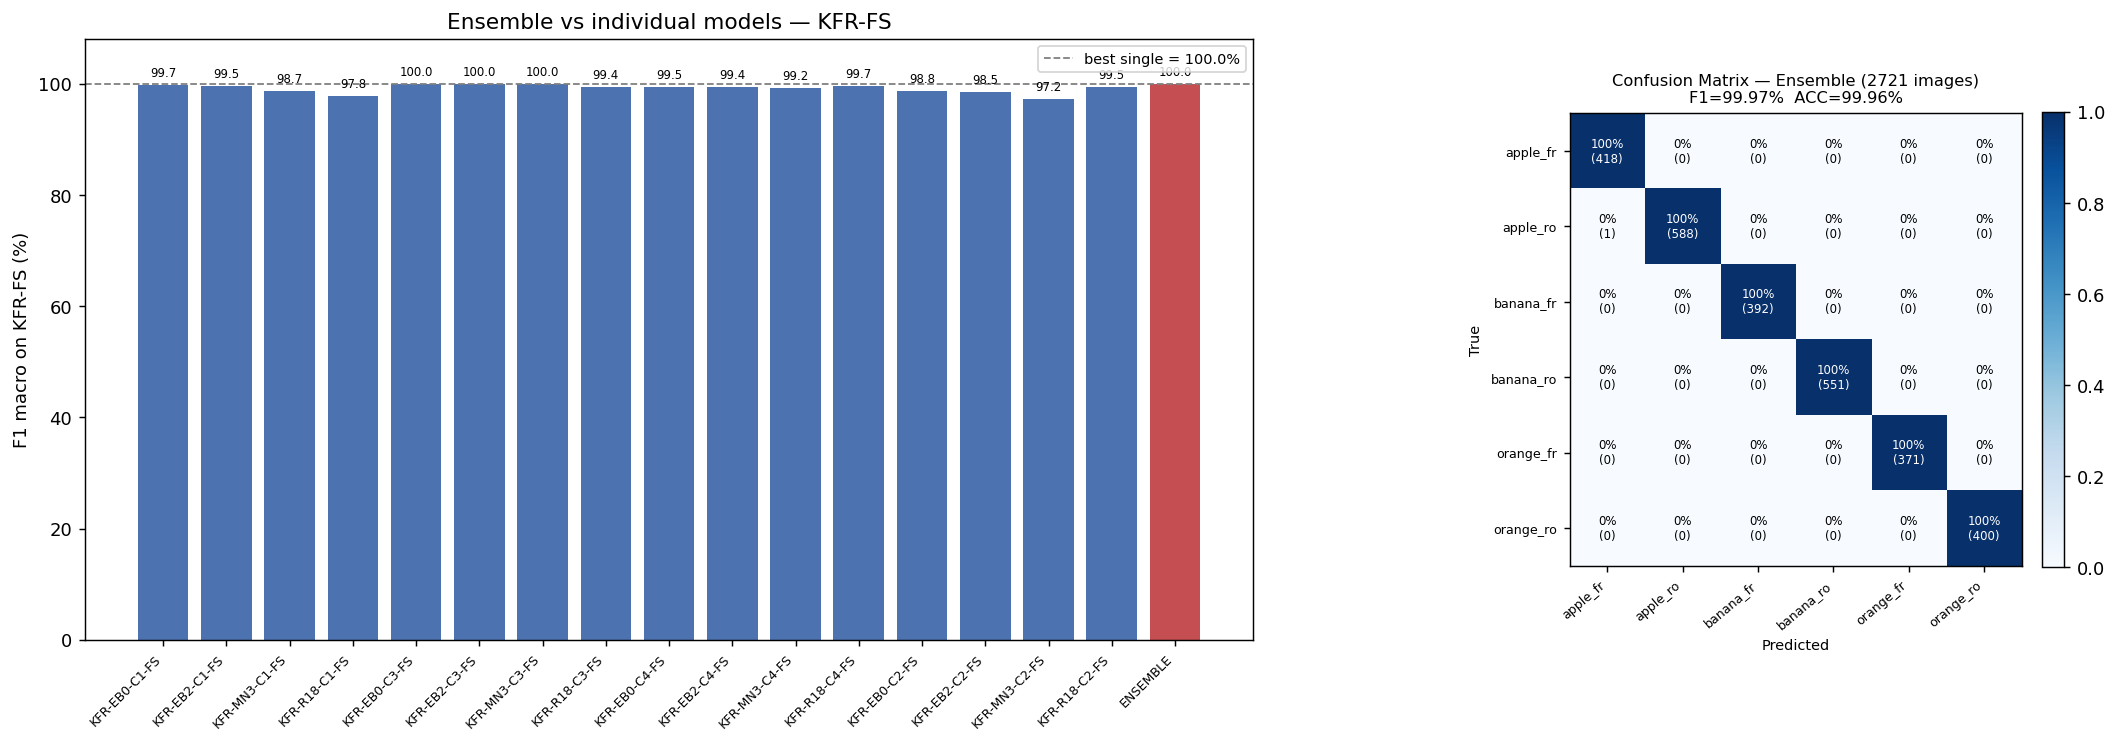
\includegraphics[width=\textwidth]{ensemble_kfr.png}
\caption{KFR fruit\_state ensemble (16 models, mean softmax).
Left: macro F1 of each individual model and the ensemble.
Right: row-normalized confusion matrix of the ensemble (percentages and counts),
showing an essentially perfect diagonal.}
\label{fig:ens_kfr}
\end{figure}

\begin{figure}[h]
\centering
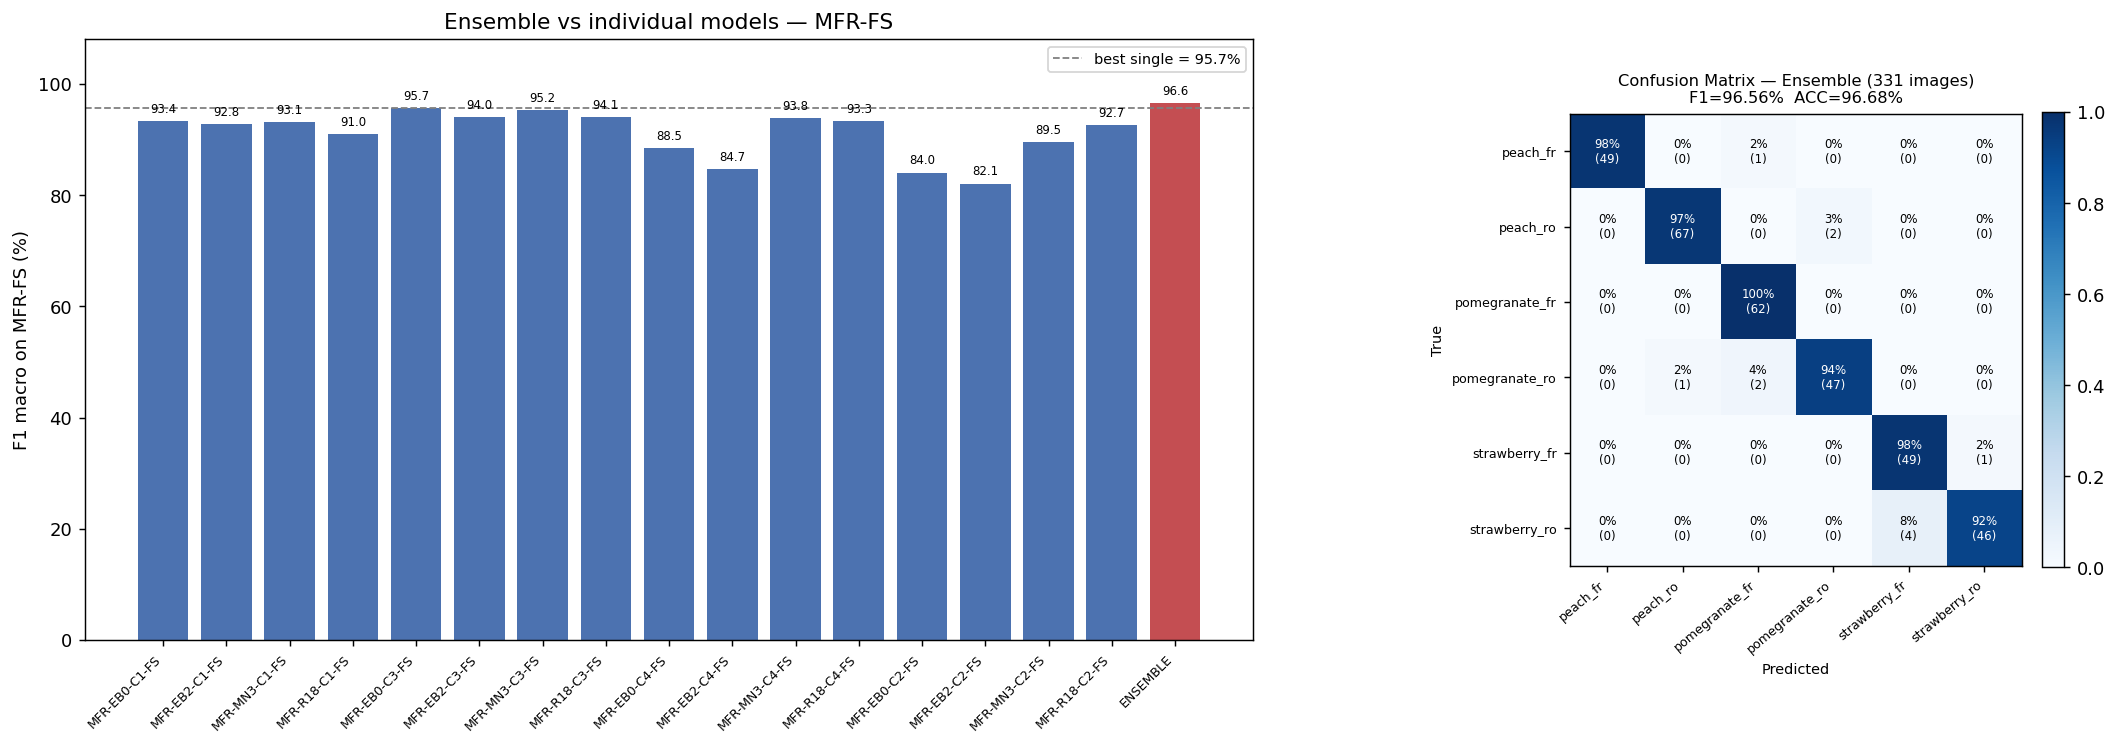
\includegraphics[width=\textwidth]{ensemble_mfr.png}
\caption{MFR fruit\_state ensemble (16 models, mean softmax).
The residual off-diagonal mass concentrates on the visually similar
pomegranate/strawberry rotten states, consistent with the lower per-class F1
on those categories.}
\label{fig:ens_mfr}
\end{figure}

\subsection{Confusion Matrix Analysis}

Figure~\ref{fig:cm} shows the row-normalized confusion matrices for two
representative completed experiments.

\begin{figure}[h]
\centering

\includegraphics[width=\textwidth]{confusion_matrix.png}
\caption{Row-normalized confusion matrices (final epoch).
The formalin class in FruitVision shows the highest misclassification rate,
predominantly confused with fresh --- analogous to the challenge of detecting
subtle spoilage in Korean fermented foods.
The Kaggle Fruits Fresh/Rotten matrix (6 classes, fruit\_state mode) shows
near-perfect diagonal structure with essentially no cross-fruit confusion.}
\label{fig:cm}
\end{figure}

\subsection{Learning Curves}

Figures~\ref{fig:acc}--\ref{fig:recall} show the per-epoch metrics for all
completed runs, grouped by dataset.
Each curve corresponds to one training condition and backbone combination.

\begin{figure}[h]
\centering
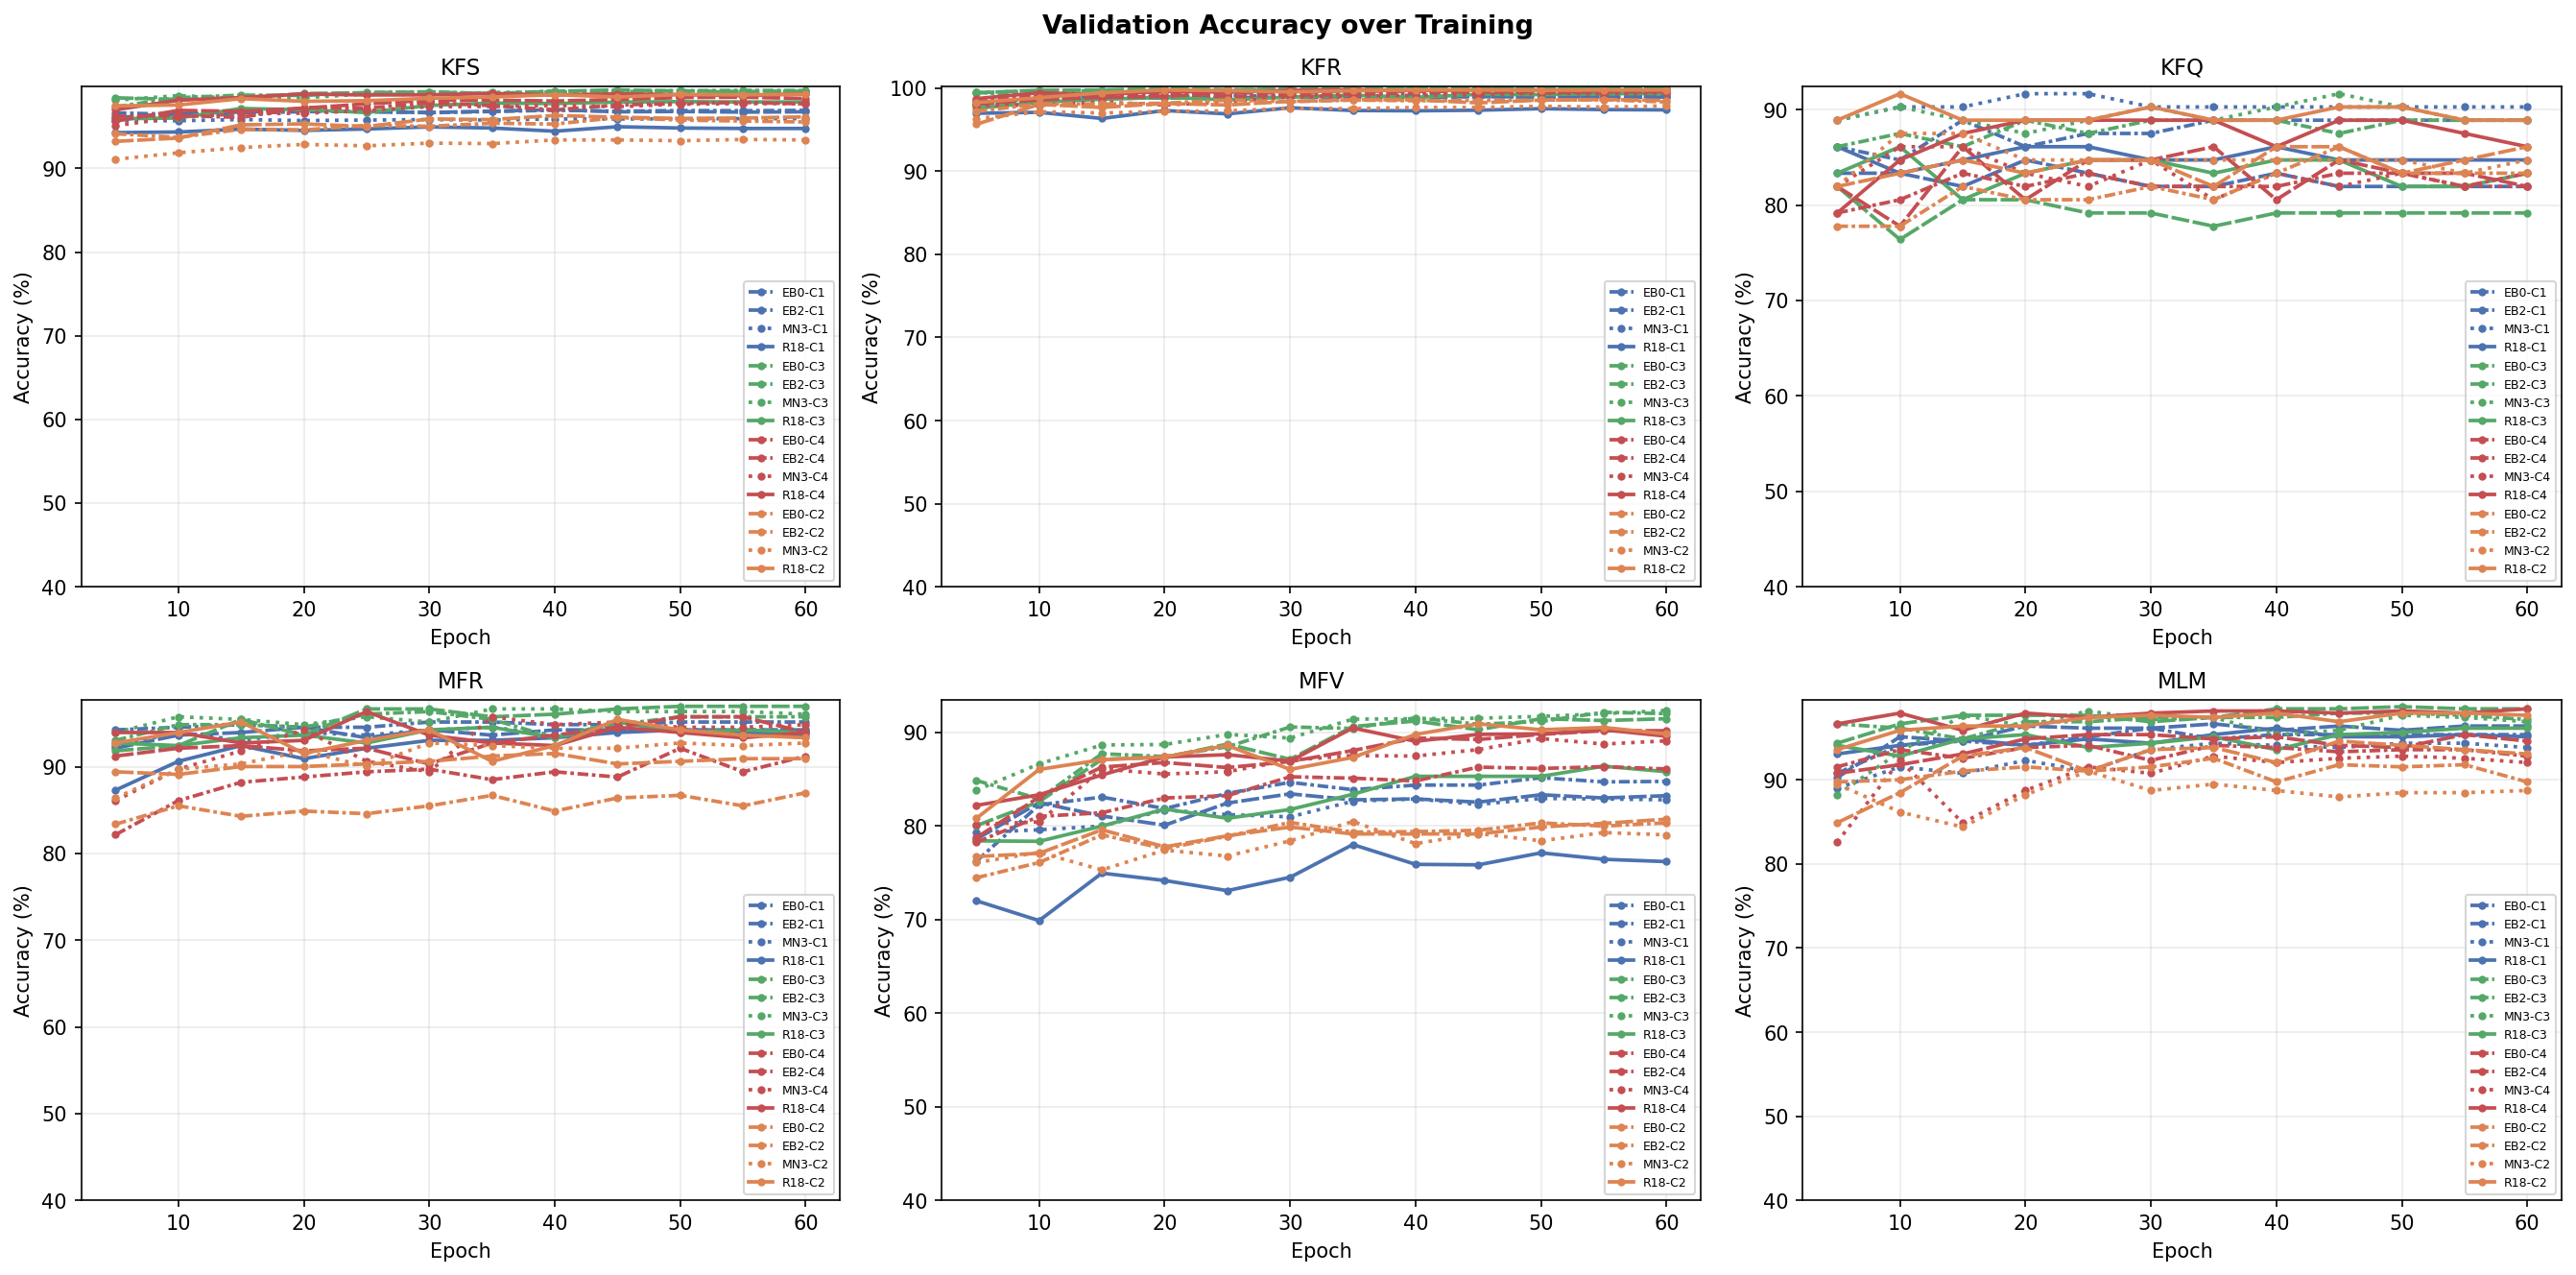
\includegraphics[width=\textwidth]{acc_curves.png}
\caption{Validation accuracy over training epochs per dataset.}
\label{fig:acc}
\end{figure}

\begin{figure}[h]
\centering
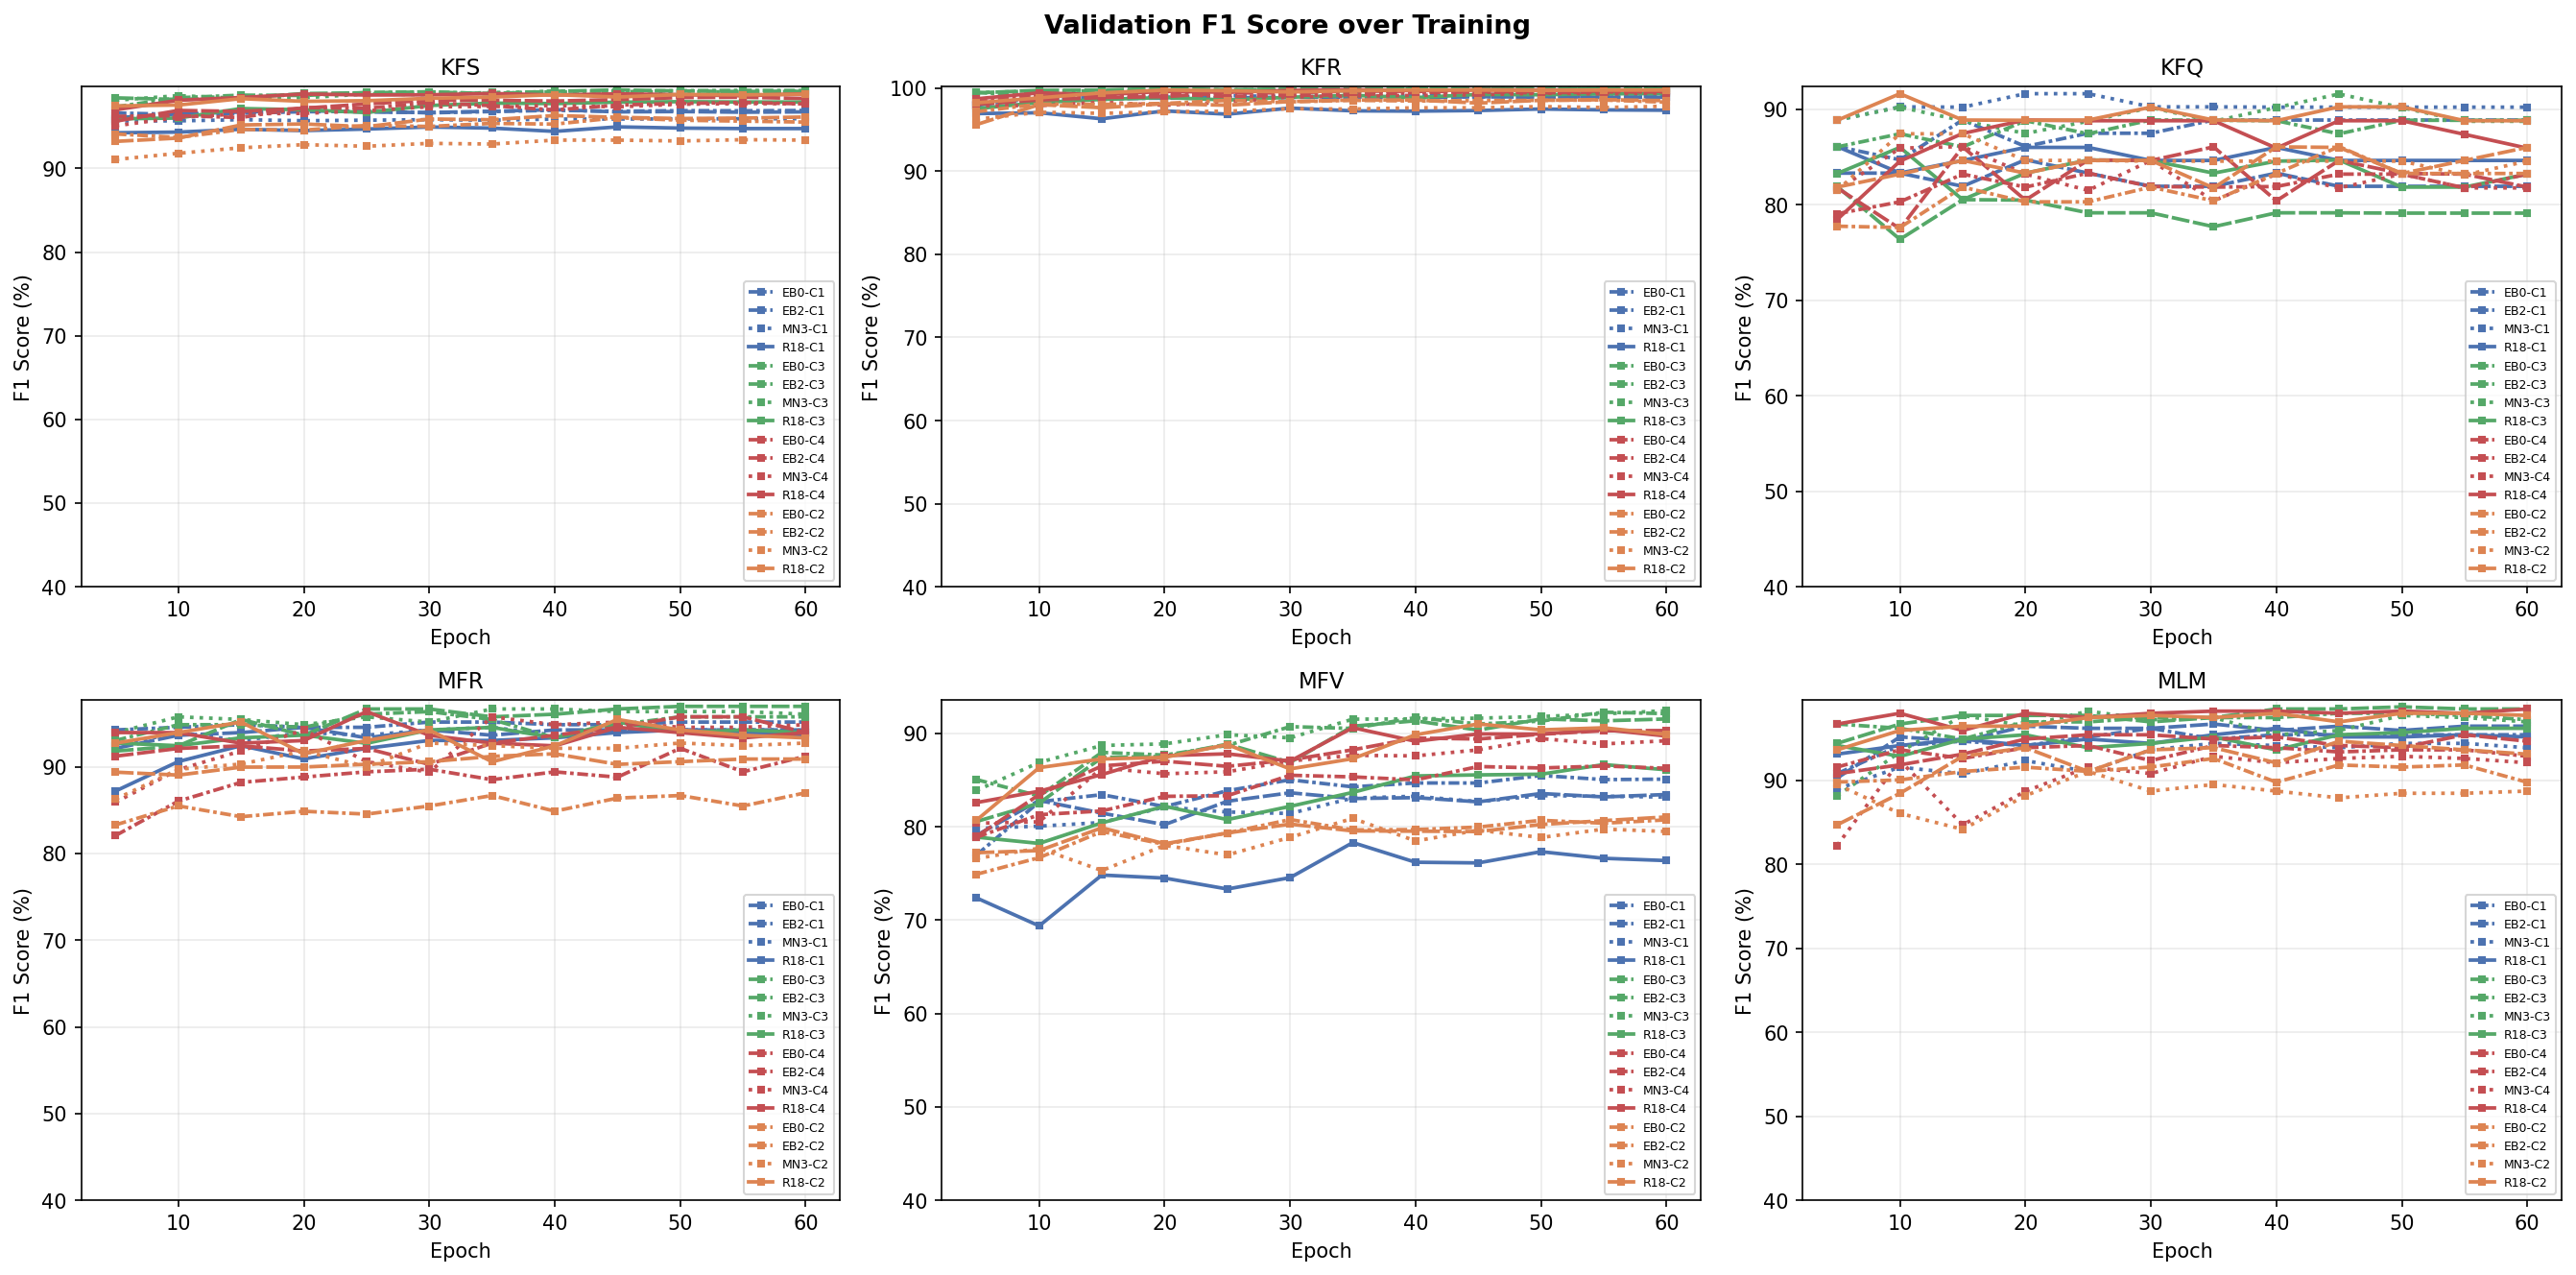
\includegraphics[width=\textwidth]{f1_curves.png}
\caption{Macro-averaged F1 score over training epochs per dataset.}
\label{fig:f1}
\end{figure}

\begin{figure}[h]
\centering
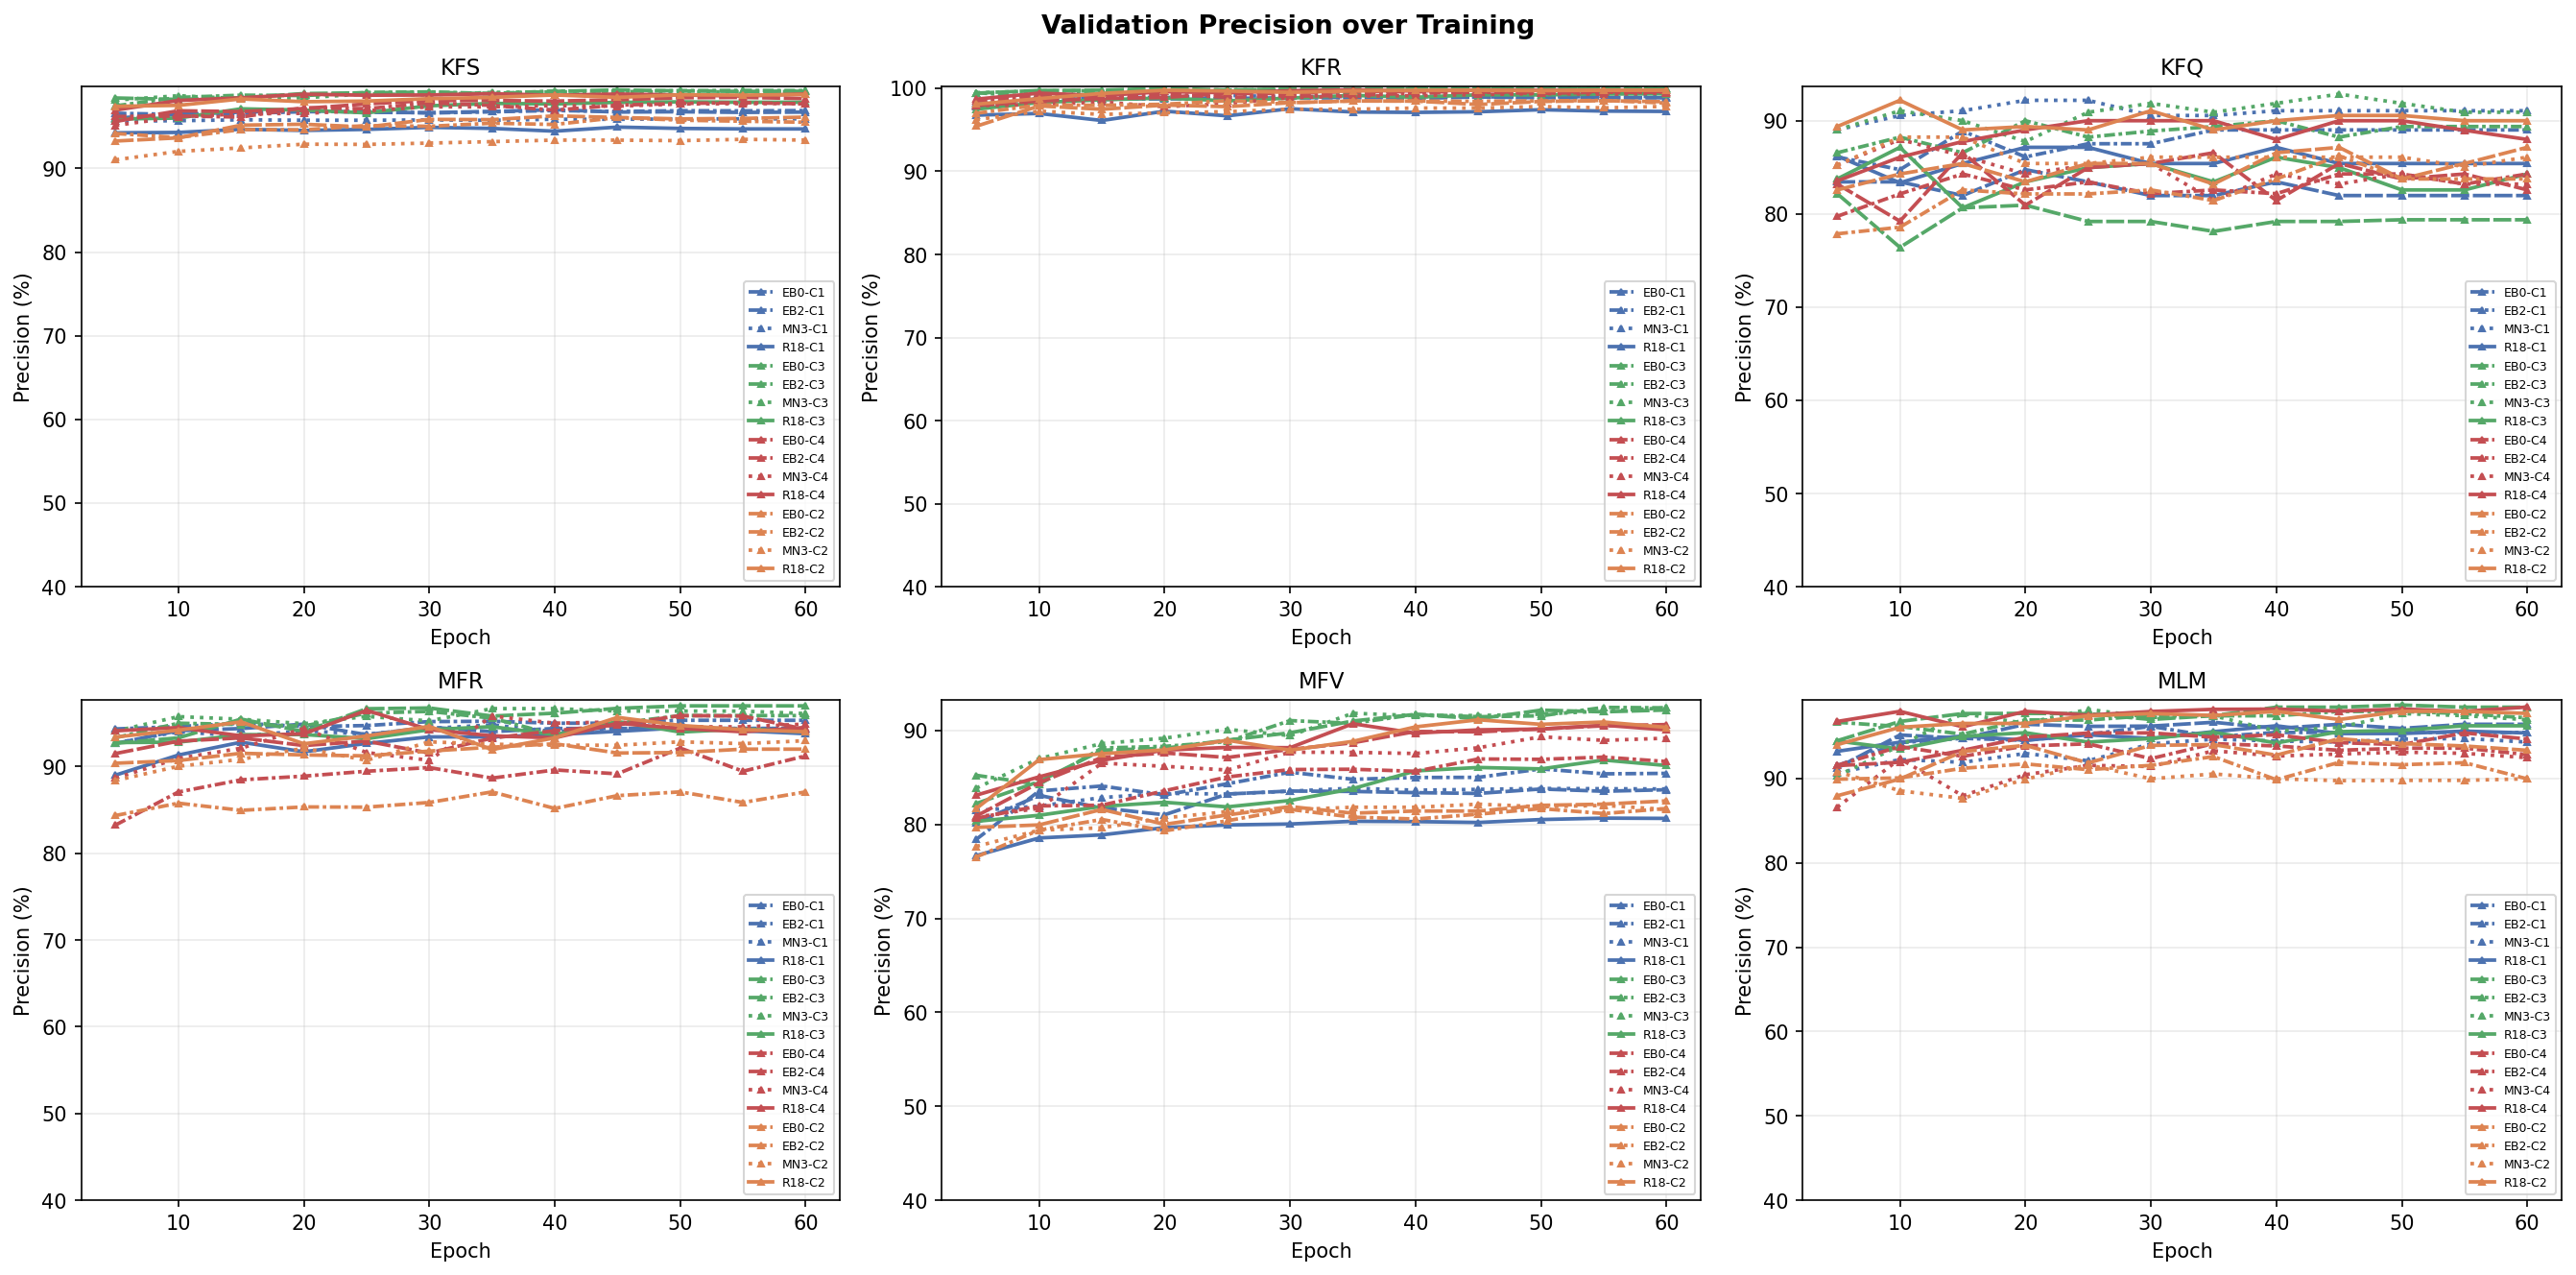
\includegraphics[width=\textwidth]{precision_curves.png}
\caption{Macro-averaged precision over training epochs per dataset.}
\label{fig:prec}
\end{figure}

\begin{figure}[h]
\centering
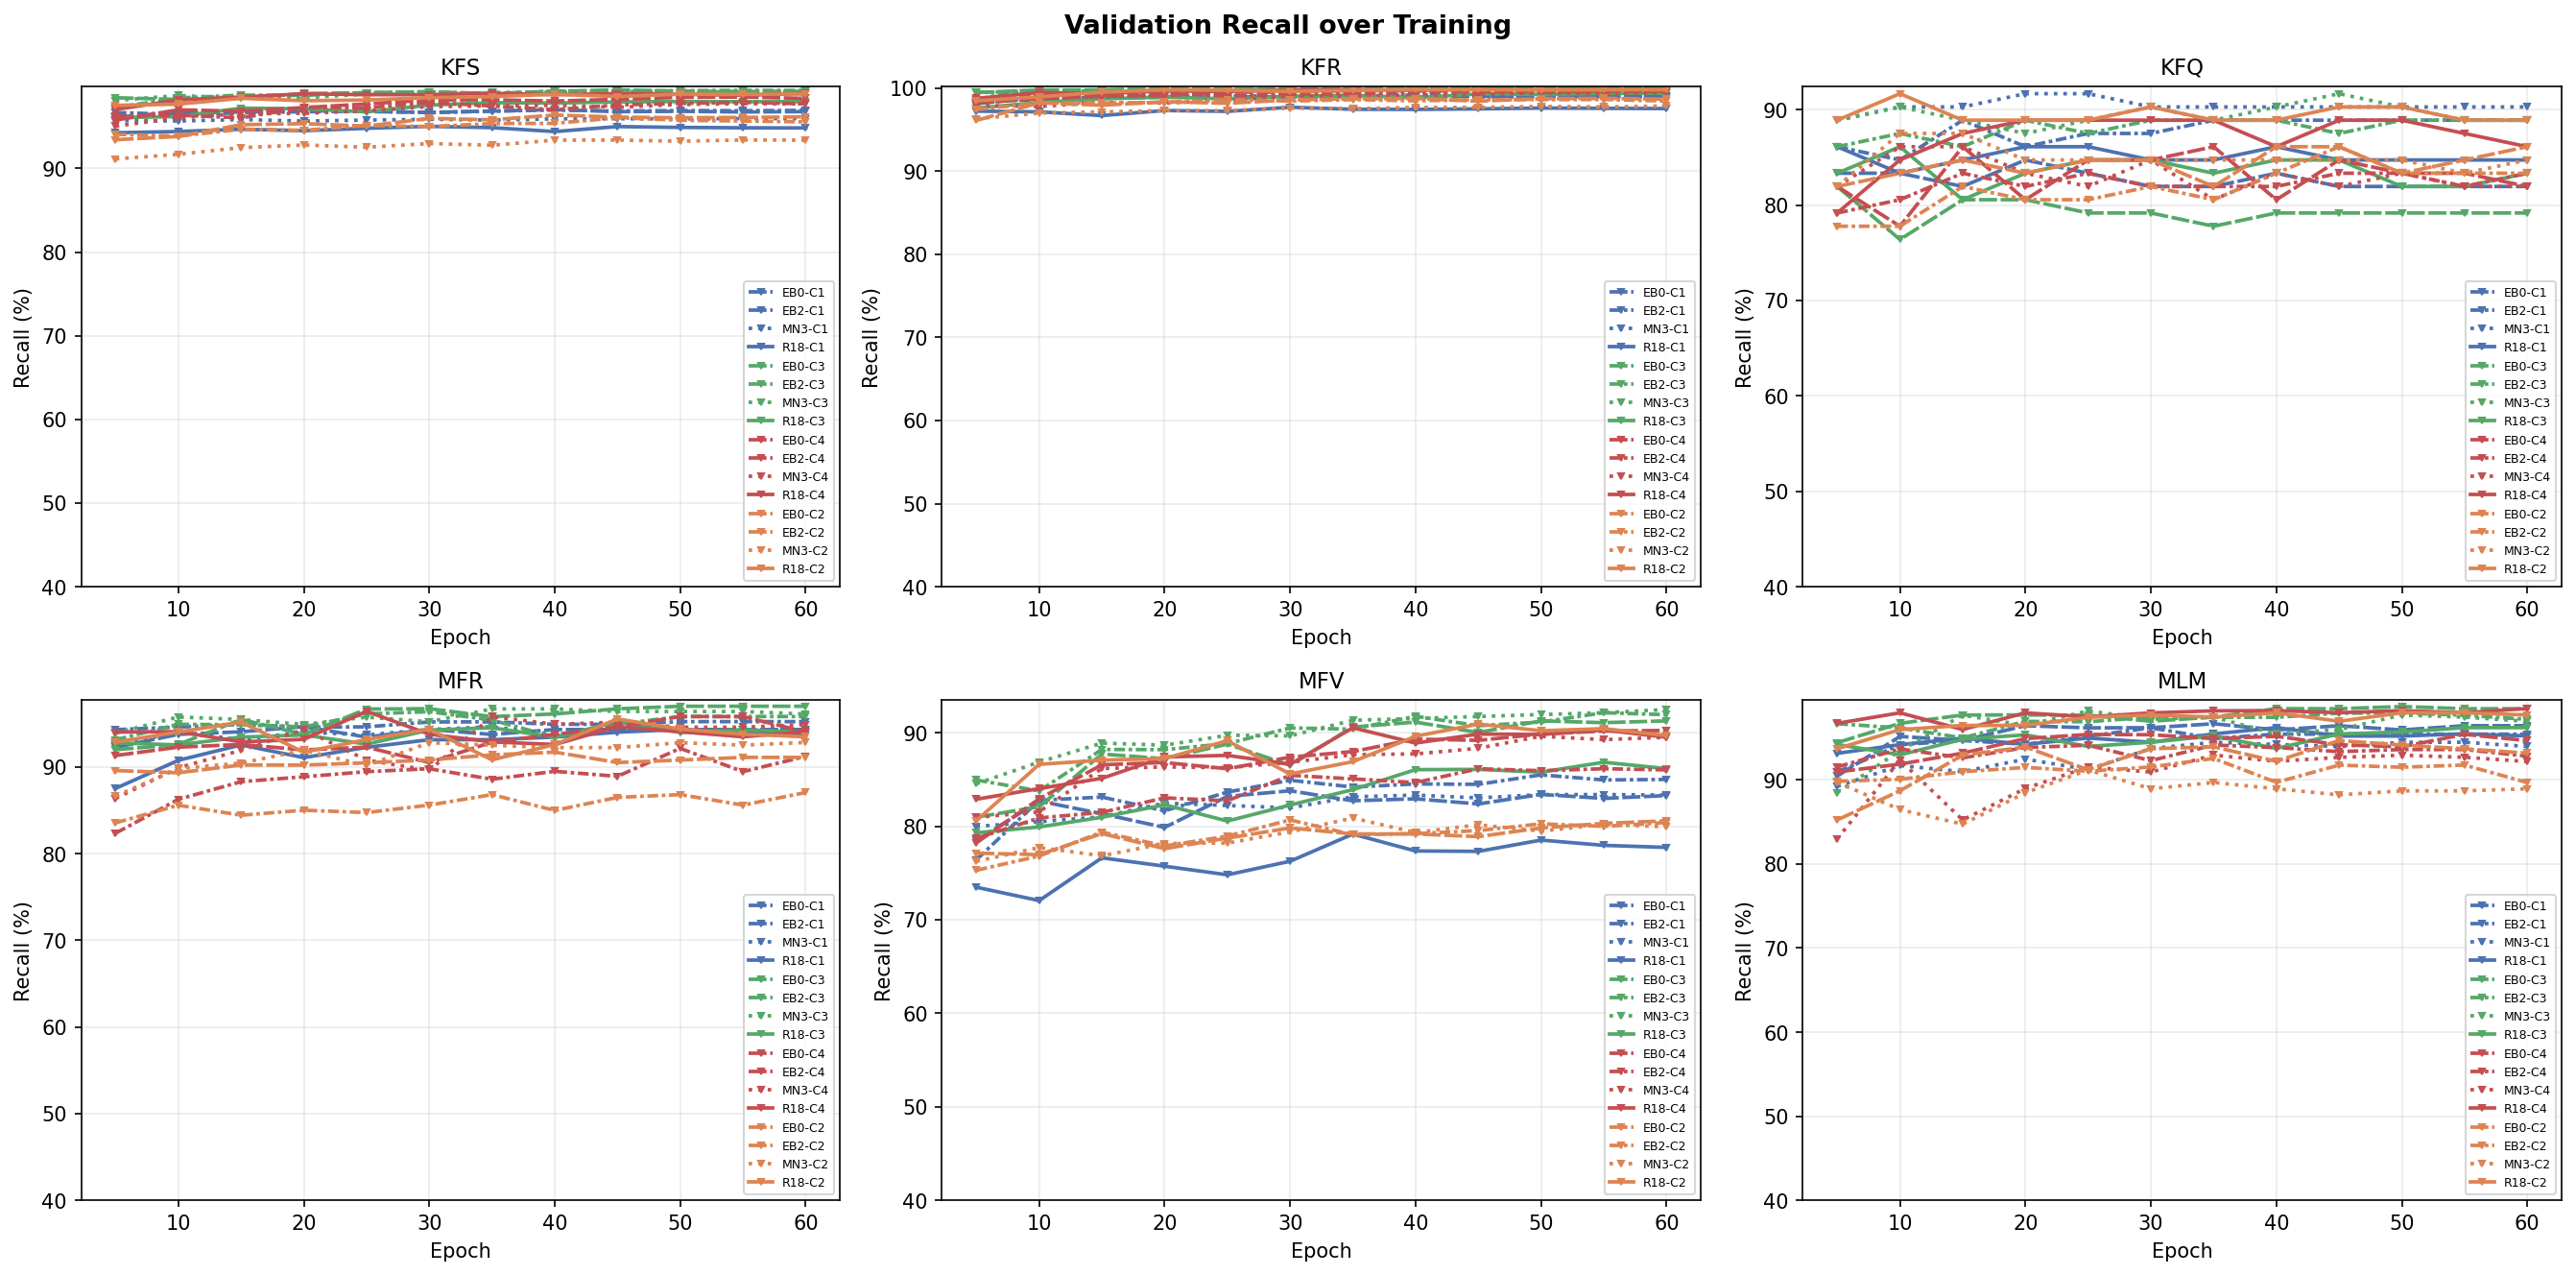
\includegraphics[width=\textwidth]{recall_curves.png}
\caption{Macro-averaged recall over training epochs per dataset.}
\label{fig:recall}
\end{figure}


\subsection{Domain Shift on Real Photos and Per-Fruit Analysis}
\label{sec:ownphotos}

To measure domain shift, trained models are evaluated on \texttt{own\_dataset},
a collection of 219 real photos taken with a phone camera under natural lighting:
121 strawberry images (64 fresh, 57 rotten) and 98 banana images
(46 fresh, 52 rotten).
This set is used \emph{only} for evaluation --- never for training --- and every
photo is scored (no held-out split).

\paragraph{Per-fruit generalization tracks training exposure.}
Because \texttt{own\_dataset} now contains two fruits, evaluation can be broken
down per fruit (\texttt{03\_05\_per\_fruit.py}).
Across all 80 evaluated state-mode models a clear pattern emerges
(Table~\ref{tab:perfruit}): a model's accuracy on a given fruit depends heavily
on whether that fruit appeared in its training data.
Models whose source dataset \emph{included} banana (e.g.\ KFR, KFS, Fruits
Quality) average 71.4\% F1 on banana, whereas models that \emph{never saw}
banana (e.g.\ Lemon Varieties, peach/pomegranate/strawberry) collapse to 42.0\%
--- barely above chance for the binary task.
Strawberry F1 is essentially unaffected ($\approx$\,80\% either way), because the
spoilage cues for strawberry transfer more readily.

\begin{table}[h]
\centering
\caption{Per-fruit F1 on own\_dataset (219 photos, state mode), averaged over
the 80 evaluated models, grouped by whether banana was seen during training.}
\label{tab:perfruit}
\setlength{\tabcolsep}{6pt}
\begin{tabular}{L{5.0cm} C{1.6cm} C{2.2cm} C{2.4cm}}
\toprule
\textbf{Model group} & \textbf{\# models} & \textbf{Banana F1} & \textbf{Strawberry F1} \\
\midrule
Saw banana in training      & 48 & \textbf{71.4} & 80.5 \\
Did not see banana          & 32 & 42.0 & 79.9 \\
\bottomrule
\end{tabular}
\end{table}

The best all-round model is EfficientNet-B0--C3 trained on Fresh\,\&\,Stale
(banana 78\%, strawberry 93\%, 86.7\% overall), reflecting that the broadest and
largest training set transfers best to unseen photographic conditions.
A per-image error analysis (\texttt{03\_04\_error\_analysis.py}) over the same
219 photos and 80 models finds an accuracy ceiling of 100\% with zero images
misclassified by every model, confirming there are no inherently unlabelable
photos --- every image is correctly handled by at least one model.

\paragraph{Domain-adaptation fine-tuning.}
The domain gap can be closed cheaply.
Taking the EfficientNet-B0 head trained on Fruits Quality (KFQ-EB0-C1-ST) as a
starting point, the classifier head was fine-tuned on \texttt{own\_dataset} with
the backbone kept frozen (30 epochs, $\text{lr}_\text{head} = 5\times10^{-4}$,
batch size 16), evaluated with 5-fold cross-validation.
Macro F1 rises from a baseline of \textbf{86.3\%} to \textbf{94.5\%}
($+8.2$ pts), with the recall on the safety-critical rotten class improving in
step.
Because only the lightweight head is updated, this adaptation requires seconds of
training and no backbone storage, making it a practical recipe for the eventual
Korean food deployment: train on abundant public images, then fine-tune the head
on a small set of in-domain photos.

% ─────────────────────────────────────────────────────────────────────────────
\section{Korean Food Dataset Proposal}
% ─────────────────────────────────────────────────────────────────────────────

\subsection{Data Collection Pipeline}

Two automated image collection scripts have been implemented, one targeting
Korean fruits and one targeting Korean prepared foods.
Both use Bing Image Search with 5--8 search queries per class per freshness
state, combining Korean-language and romanized search terms to maximize
result diversity (e.g., \textit{``fresh kimchi bright red color''} and
\textit{``moldy kimchi white fungus''} for the kimchi category).

Downloaded images are validated and processed as follows:
\begin{itemize}
    \item \textbf{Integrity check}: corrupt or unreadable files are discarded.
    \item \textbf{Minimum resolution}: $100 \times 100$ pixels.
    \item \textbf{Format}: any format accepted; converted to RGB JPEG.
    \item \textbf{Output size}: $256 \times 256$ pixels
    (model crops to $224 \times 224$ during training).
\end{itemize}

\subsection{Integration with Training Pipeline}

The Korean food dataset will be organized in the same
\texttt{food/state/} nested structure used throughout this study,
making it directly compatible with the existing training and evaluation
pipeline without any code modifications.
The \texttt{prepare\_datasets.py} script can be extended with a new
preparation function, and the training pipeline selects the dataset
interactively at runtime.

% ─────────────────────────────────────────────────────────────────────────────
\section{Software Implementation}
\label{sec:sw}
% ─────────────────────────────────────────────────────────────────────────────

The classification system is implemented in Python (PyTorch) and organized into
four numbered stages (data preparation, training, evaluation/analysis, and
reporting) plus two internal libraries.
Figure~\ref{fig:pipeline} illustrates the data flow between components.

\subsection{Usage Workflow}

Scripts are organized in four numbered stages.
Internal libraries (\texttt{\_backbone.py}, \texttt{\_dataset.py}) are
imported automatically and never run directly.

\begin{enumerate}
    \item \textbf{Stage 01 --- Data preparation}
    \texttt{01\_01\_prepare\_datasets.py} reorganizes raw datasets into the
    unified \texttt{data/\{dataset\}/\{fruit\}/\{state\}/} structure.
    \texttt{01\_02\_rename\_own\_dataset.py} and
    \texttt{01\_03\_prepare\_own\_dataset.py} handle own photos.

    \item \textbf{Stage 02 --- Training}
    \texttt{02\_01\_train.py} presents an interactive menu to select dataset,
    label mode, condition, and backbone.
    Results are saved to \texttt{run\_outputs/\{run\_name\}/}.

    \item \textbf{Stage 03 --- Evaluation and analysis}
    \texttt{03\_01\_evaluate.py} loads any \texttt{best\_model.pt} and
    evaluates it on any dataset, generating per-image predictions and plots.
    \texttt{03\_02\_analyze.py} reads all \texttt{metrics.json} files and
    generates training-curve comparison plots.
    \texttt{03\_03\_ensemble.py} combines several models' per-image
    probabilities into an ensemble (mean / weighted / adaptive) for any dataset
    and label mode, with a confusion-matrix plot.
    \texttt{03\_04\_error\_analysis.py} ranks individual photos by how many
    models misclassify them, and \texttt{03\_05\_per\_fruit.py} breaks the
    own\_dataset evaluation down per fruit.

    \item \textbf{Stage 04 --- Reporting}
    \texttt{04\_01\_generate\_tracker.py} produces
    \texttt{04\_01\_experiments\_tracker.xlsx} with color-coded run status.
    \texttt{04\_02\_generate\_eval\_report.py} produces
    \texttt{04\_02\_eval\_report.xlsx} with ranked cross-dataset results.
    \texttt{04\_03\_generate\_own\_report.py} consolidates the own\_dataset
    domain-adaptation findings (fine-tuning, per-fruit, error analysis, ensemble)
    into \texttt{04\_03\_own\_dataset\_report.xlsx}, and
    \texttt{04\_04\_generate\_benchmark\_report.py} builds
    \texttt{04\_04\_benchmark\_report.xlsx} comparing our models against the
    published papers of Section~\ref{sec:fruitstate}.
    Domain-adaptation fine-tuning itself is performed by
    \texttt{02\_02\_finetune.py}.
\end{enumerate}

\begin{figure}[h]
\centering
\begin{tabular}{ccccc}
\fbox{\texttt{datasets/}} & $\longrightarrow$ &
\fbox{\texttt{01\_01\_prepare\_datasets.py}} & $\longrightarrow$ &
\fbox{\texttt{data/}} \\[6pt]
& & & & $\downarrow$ \\[6pt]
\fbox{\texttt{\_backbone.py}} & $\longrightarrow$ &
\multicolumn{3}{c}{\fbox{\texttt{02\_01\_train.py}  $\longleftarrow$  \texttt{\_dataset.py}}} \\[6pt]
& & & & $\downarrow$ \\[6pt]
& & \multicolumn{3}{c}{\fbox{\texttt{run\_outputs/\{run\_name\}/}}} \\[6pt]
& & & & $\downarrow$ \\[6pt]
\fbox{\shortstack{\texttt{03\_01\_evaluate}\\\texttt{03\_03\_ensemble}}} & $\longrightarrow$ &
\multicolumn{3}{c}{\fbox{\shortstack{
\texttt{03\_02\_analyze} $\to$ \texttt{run\_outputs/\_plots/}\\
\texttt{04\_0x\_generate\_*} $\to$ \texttt{*.xlsx} reports}}}
\end{tabular}
\caption{Data flow across the four numbered stages.
Internal libraries (\texttt{\_backbone.py}, \texttt{\_dataset.py}) are imported,
never run directly.}
\label{fig:pipeline}
\end{figure}

\subsection{\texttt{prepare\_datasets.py} --- Dataset Preparation}

Raw datasets are downloaded from their respective sources and placed in the
\texttt{datasets/} directory, each in its original folder structure.
\texttt{prepare\_datasets.py} reads each raw dataset and reorganizes it into
a unified \texttt{data/\{dataset\}/\{fruit\}/\{state\}/} hierarchy compatible
with PyTorch's \texttt{ImageFolder} loader.
The script handles format differences across datasets:
flat structures (all images in one folder), split structures (pre-divided
\texttt{train/test/}), and nested structures (fruit then state sub-folders).
Each dataset has a dedicated preparation function that normalizes class names,
resolves naming inconsistencies (e.g.\ \texttt{freshpatato}
$\to$ \texttt{potato/fresh}), and copies or hard-links images to the output
directory.
The script is idempotent: re-running it on an already-prepared dataset
overwrites nothing.

\subsection{\texttt{backbone.py} --- Backbone Registry}

A central registry (\texttt{BACKBONE\_REGISTRY}) maps string identifiers
(\texttt{"resnet18"}, \texttt{"efficientnet\_b0"}, etc.) to factory functions
that return pre-trained models loaded from \texttt{torchvision}.
The \texttt{GenericBackbone} wrapper exposes a unified interface:
\begin{itemize}
    \item \texttt{forward(x)} returns the feature vector of dimension
    $d_\text{out}$ (the output of the backbone's global pooling layer,
    \emph{before} the original classification head).
    \item \texttt{unfreeze\_layers(n)} selectively unfreezes the last $n$
    layer groups of the backbone, leaving all earlier weights frozen.
    For ResNet this corresponds to the last $n$ residual stages
    (\texttt{layer4}, \texttt{layer3}, \ldots).
\end{itemize}
This design decouples the backbone choice from the training loop, making it
trivial to swap architectures.

\subsection{\texttt{dataset.py} --- Data Loading}

\texttt{dataset.py} provides three loaders that cover the three folder layouts
found across the six datasets:
\begin{itemize}
    \item \textbf{Layout A} (flat): all images in a single directory.
    \item \textbf{Layout B} (split): pre-divided \texttt{train/} and
    \texttt{test/} sub-folders.
    \item \textbf{Layout C} (nested): \texttt{fruit/state/} hierarchy,
    used for all experiments in this study.
\end{itemize}
For Layout C, \texttt{get\_loaders\_nested()} constructs a stratified 80/20
train/validation split using scikit-learn's \texttt{StratifiedShuffleSplit}.
Two separate \texttt{ImageFolder} objects (one with augmentation transforms,
one with validation-only transforms) are created over the same index sets so
that training and validation images receive different preprocessing.
The \texttt{label\_mode} parameter controls whether class labels are derived
from freshness state only (\texttt{state}) or from fruit-state combinations
(\texttt{fruit\_state}).

\subsection{\texttt{train.py} --- Training Loop}

The training script presents an interactive menu for dataset, label mode,
condition, and backbone selection.
The run directory name is deterministically computed from these choices
(e.g.\ \texttt{mendeley\_fruitvision\_all\_head\_layer4\_resnet18\_fs}),
which serves as both a unique identifier and a resume key.

Training proceeds for a fixed number of epochs (default 50) with the following
behavior:
\begin{itemize}
    \item \textbf{Evaluation every 5 epochs}: accuracy, macro F1, macro
    precision, macro recall, per-class metrics, and confusion matrix are
    computed on the validation set and appended to \texttt{metrics.json}.
    \item \textbf{Rolling checkpoint every 10 epochs}: a single
    \texttt{checkpoint.pt} file is overwritten, keeping disk usage constant.
    \item \textbf{Best model}: whenever validation F1 improves, the full model
    state is saved to \texttt{best\_model.pt}.
    \item \textbf{Resume}: if a checkpoint exists in the run directory,
    training automatically resumes from the last saved epoch.
\end{itemize}
At the end of training, all metrics are serialized to
\texttt{metrics.json}, which serves as the single source of truth for all
subsequent analysis.

\subsection{\texttt{analyze.py} --- Visualization}

\texttt{analyze.py} scans \texttt{run\_outputs/} for all
\texttt{metrics.json} files, loads them into a list of run records, and
generates nine plots grouped into three categories.

\textbf{Learning curves} (one subplot per dataset, one line per
condition+backbone combination):
\begin{itemize}
    \item \texttt{acc\_curves.png} --- validation accuracy vs.\ epoch.
    Shows whether training has converged and whether different conditions
    converge at different rates.
    \item \texttt{f1\_curves.png} --- macro F1 vs.\ epoch.
    The primary metric used for model selection; reveals overfitting when
    F1 peaks and then declines.
    \item \texttt{precision\_curves.png} --- macro precision vs.\ epoch.
    Indicates how often the model's positive predictions are correct.
    \item \texttt{recall\_curves.png} --- macro recall vs.\ epoch.
    Indicates how many true positives the model captures; particularly
    important for the rotten and formalin classes.
    \item \texttt{loss\_curves.png} --- training loss and validation loss
    vs.\ epoch on the same axes.
    Divergence between the two signals overfitting.
\end{itemize}

\textbf{Aggregate comparisons} (summarize best results across all runs):
\begin{itemize}
    \item \texttt{metrics\_summary.png} --- grouped bar chart showing the
    best macro F1, precision, recall, and accuracy for each run, organized
    by dataset and condition.
    Useful for a quick overview of which configuration wins.
    \item \texttt{heatmap.png} --- a condition $\times$ backbone grid where
    each cell shows the best F1 achieved.
    Empty cells correspond to experiments not yet run.
\end{itemize}

\textbf{Error analysis} (inspect what the model gets wrong):
\begin{itemize}
    \item \texttt{confusion\_matrix.png} --- row-normalized confusion matrix
    for each completed run at the final epoch.
    Each row represents a true class; each column a predicted class.
    Values on the diagonal are correct classifications; off-diagonal values
    reveal systematic confusions (e.g.\ formalin predicted as fresh).
    \item \texttt{per\_class.png} --- bar chart of F1, precision, and recall
    broken down by individual class for each run.
    Identifies which specific class is pulling the macro average down.
\end{itemize}

All plots are saved to \texttt{run\_outputs/\_plots/}.
Running \texttt{prepare\_figures.py} copies them --- together with the ensemble
confusion matrices from \texttt{run\_outputs/\_ensemble/} and the per-fruit
breakdown --- into \texttt{figures/} for inclusion in this report.

\end{document}
